\chapter{QAM信号量子接收机}
在上一章中,我们回顾了现有的一些量子接收机实现方案,
包括二元检测和多元的PSK和PPM检测量子接收机。
但是到目前为止,专门针对QAM信号设计的量子接收机
研究还比较少。然而,QAM信号具有很高的频谱效率,
已被应用到大容量光通信系统之中\cite{winzer2012high}。
因此,研究QAM信号量子接收机是一件很有必要的事情。

\section{QAM信号接收机理论极限}
\subsection{标准量子极限}
在经典通信系统中,常用外差接收机检测QAM信号,
这种接收机的性能也叫QAM信号的标准量子极限(SQL)\cite{kato1999quantum}。
设$M$阶QAM信号由$M$个相干态构成,如图\ref{fig:QAM-signals}所示,
显示的是16-QAM和36-QAM星座图。假设$M$阶QAM信号每一个
正交幅度$X$或$P$都可以取$L$个不同的值,那么$M=L^2, L=3,4,5...$。
设这$L$元基本符号集合为$\Omega = \{-(L-1) + 2(i-1) | i=1,2,...,L\}$,
那么$M$阶QAM信号
可以表示为
\begin{equation}
\ket{\alpha_{uv}} = \ket{\alpha(u + j v)}, (u, v) \in \Omega. 
\end{equation}
这里$j=\sqrt{-1}$。例如,16-QAM信号就可以用相干态表示为
\begin{equation}
\begin{split}
\ket{\alpha_{1,1}} &= \ket{\alpha(1 + j )}, \\
\ket{\alpha_{1,3}} &= \ket{\alpha(1 + j 3)}, \\
\ket{\alpha_{1,-1}} &= \ket{\alpha(1 - j )}, \\
                &\vdots                      \\
\ket{\alpha_{-3,-3}} &= \ket{\alpha(-3 - j 3)}.
\end{split}
\end{equation}
这里取$\alpha > 0$,那么M阶QAM信号信号平均光子数为
\begin{equation}
\begin{split}
n &= |\alpha|^2 \frac{1}{M}\sum_{u \in \Omega}\sum_{v \in \Omega} (u^2+v^2)\\
  &= \frac{2}{3}(M-1) |\alpha|^2.
\end{split}
\end{equation}


\begin{figure}
\centering
  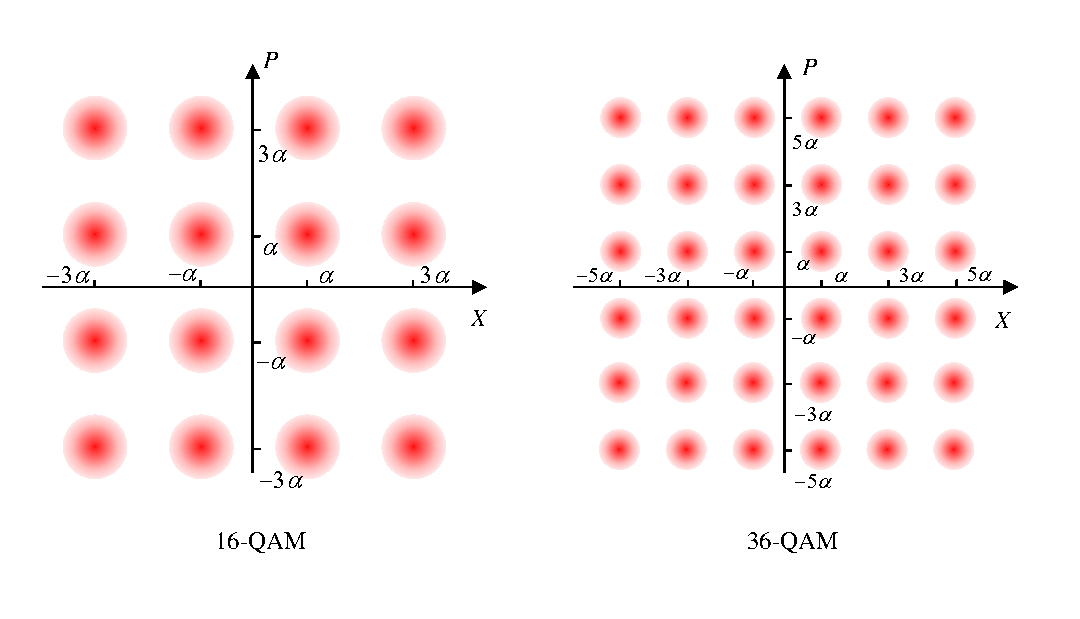
\includegraphics[width=0.8\textwidth]{figures/chap3/QAM-signals}
  \caption{QAM信号星座图}
  \label{fig:QAM-signals}
\end{figure}


下面我们来计算一下QAM信号的标准量子极限。
利用式\ref{eq:Her-receiver-output}可得理想情况下,
外差接收机的概率密度函数为\cite{kato1999quantum}
\begin{equation}
p(x_c, x_s| u, v) = \frac{1}{\pi} \exp[-(x_c - u\alpha)^2 - (x_s - v\alpha)^2]
\end{equation}
这里$x_c$和$x_s$对应于式\ref{eq:Her-receiver-output}中的$\alpha_1$和$\alpha_2$,
是接收机输出的两个正交幅度观测量。
根据贝叶斯检测理论,最优判决区域为
\begin{equation}
D_{u',v'} = \{ (x_c,x_s)| D_L(u') < x_c \le D_U(u'),  D_L(v') < x_s \le D_U(v') \}
\end{equation}
这里$D_U$和$D_L$是两个上下界函数,对给定的参数$L$,
定义为
\begin{equation}
\begin{split}
D_L(u) &= \begin{cases}    
          -\infty     & u < -(L-2)  \\
          \alpha(u-1) & otherwise
         \end{cases}\\
D_U(u) &= \begin{cases} 
          \infty     & u > L-2  \\
          \alpha(u+1) & otherwise
         \end{cases}
\end{split}
\end{equation}
即将复平面划分成如图\ref{fig:QAM-domain-split}所示的$M$个判决
区域,将输出统计量落在某个区域的结果判决为在该区域内的符号。
那么,外差接收机的平均错误概率为
\begin{equation}
\begin{split}
P_e &= 1 - \frac{1}{M} \sum_{u\in\Omega}\sum_{v\in\Omega} \iint_{D_{u,v}} p(x_c,x_s|u,v) dx_c dx_s \\
    &= 1 - \frac{1}{M}[1+(L-1) \erf(\alpha)]^2.
\end{split}
\end{equation}
因此,当平均光子数很大时,即$|\alpha|^2 \gg 1$,
利用余误差函数的Chernoff界\cite{chang2011chernoff},
可得QAM信号外差接收机的渐近性能为
\begin{equation}
\begin{split}
P_e &\approx 2\frac{L-1}{L} e^{-\alpha^2}.
\end{split}
\end{equation}

\begin{figure}
\centering
  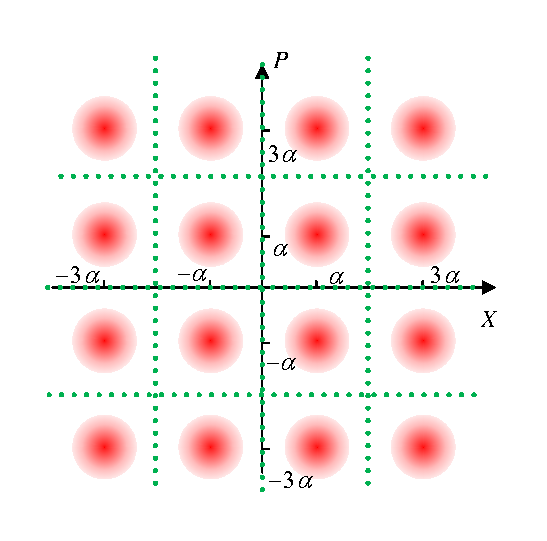
\includegraphics[height=5cm]{figures/chap3/QAM-domain-split}
  \caption{16-QAM信号外差接收判决区域划分示意图}
  \label{fig:QAM-domain-split}
\end{figure}

\subsection{Helstrom极限}
与PSK信号和PPM信号不同的是,QAM信号不再具有几何均匀对称性,
因此,无法通过平方根检测的方法得到QAM信号Helstrom极限的解析表达式,
需要通过数值优化的方法,求解优化问题\ref{eq:Hel-SDP}。
为此,需要将信号用密度矩阵表示出来。
由于$M$个信号互不正交,因此这$M$个信号张成$M$维Hilbert空间。
因为是纯态信号,所以每一个信号都可以用一个向量表达。
为此需要选择一组标准正交基$\ket{e_i}, i=1,2,...,M$。
一种选取的方法是用Fork态做标准正交基,也可以利用Smit正交化的方法
生成一组基向量\cite{zxd2004matrix}。
这里,为方便计我们选用Fork态$\ket{n}$作为标准正交基,在这组基向量下,
每一个信号都是一个无穷维向量,
\begin{equation}
c_n = \bra{n}\ket{\alpha} = e^{-\frac{1}{2}|\alpha|^2} \frac{\alpha^n}{\sqrt{n!}}.
\end{equation}
它满足归一化条件
\begin{equation}
\sum_{n=0}^{\infty} c_n = 1.
\end{equation}
为了便于计算,需要将这个无穷维向量截断成有限维向量。
这里采用如下准则,给定一个足够小的$\epsilon$,选取截断后向量长度$l$满足
\begin{equation}
\sum_{n=0}^{l-1} c_n \ge 1 - \epsilon.
\label{eq:epsilon-criterion}
\end{equation}
例如,当$\alpha=1, \epsilon=10^{-4}$时,信号$\ket{\alpha}$可以近似表达
为一个7维向量,
\begin{equation}
\ket{\alpha} = [0.6065, \\
    0.6065, \\
    0.4289, \\
    0.2476, \\
    0.1238, \\
    0.0554, \\
    0.0226]^T.
\end{equation}
对于$M$个QAM信号集合,在计算的时候需要将每一个
信号向量$\bm{c}_i$截断成维数相同的向量$\tilde{\bm{c}}_i$。
截断后的向量长度$L$满足
\begin{equation}
\begin{split}
L = \max_i l_i  \\
s.t. \sum_{n=0}^{l_i-1} c_{in} \ge 1 - \epsilon, i=1,2,...,M.
\end{split}
\end{equation}
这里$c_{in}$代表第$i$个信号向量$\bm{c}_i$的第$n$维。
上式选取的长度$L$可以保证$M$个信号都满足式\ref{eq:epsilon-criterion}。

将信号表达为$L$维向量$\tilde{\bm{c}}$后,信号的密度矩阵可以表达为
\begin{equation}
\hat{\rho}_i = \tilde{\bm{c}} \tilde{\bm{c}}^T.
\end{equation}
接下来,我们就可以利用CVX工具箱求解半正定规划问题\ref{eq:Hel-SDP},
从而得到Helstrom极限对应的平均错误概率。





\section{QAM信号Bondurant接收机}


\section{QAM信号自适应分区检测接收机}


\section{QAM信号混合接收机}


\section{三种接收机的对比}

